\documentclass[mathserif]{beamer}

%% Packages section
\usepackage[utf8]{inputenc}
\usepackage{graphicx}
\usepackage{tikz}
%% \usepackage{caption}
\newcommand{\myfig}[2] {
  \begin{figure}[!h]
    \centering
    \includegraphics[scale=#1]{#2}
  \end{figure}
}

%% Options section
\usetheme{Boadilla} 
\useinnertheme[shadow]{rounded}
\usecolortheme{dolphin}
\useoutertheme{infolines}

\title{Monitoring du noyau Linux}
\subtitle{sur une architecture NUMA}
%% \subtitle{Sous la direction de Gaël Thomas}
\author[Gallardo - Lombardet - Peneau]{Kevin Gallardo\\Eric Lombardet\\Pierre-Yves Péneau}

\newcommand{\bframe}{\begin{frame}{\secname}{\subsecname}}

\date{12 Mai 2014} \institute[UPMC]{Université Pierre et Marie
  Curie}

\begin{document}

  %% \captionsetup[figure]{labelformat=empty}

  \frame{\titlepage}

  \chapter{Architecture des ordinateurs}

  \lettrine[nindent=0em,lines=3]{N} ous allons dans un premier temps revenir sur le fonctionnement des
  ordinateurs indépendement de l'architecture considérée. Ainsi, les différents
  concepts seront expliqués dans leur généralités avant d'exposer les
  spécificités de l'architecture NUMA. Cette partie nous permettra de faire un
  bilan général des connaissances acquises lors des modules d'architecture et de
  noyau lors de cette année.


  \section{Principes généraux}

    \subsection{Le processeur}

    Le processeur est le coeur de l'ordinateur.  Son rôle est d'effectuer tous
    les calculs, lectures et écritures sur les données. Un processeur est
    cadencé à une certaine vitesse qui se mesure en cycle et qui varie selon les
    modèles.. À chaque cycle, le processeur est chargé d'aller chercher une
    instruction dans la mémoire, la décoder et l'exécuter.

    \subsubsection{Les caches}

      L'accès à la mémoire est une opération très couteuse, entre 100 et 2000
      cycles\cite{Lepers2014}. Afin d'accélérer ce processus, les ingénieurs ont
      créé les mémoires cache, ou plus communément caches. Les caches sont une
      zone mémoire de taille infiniment inférieure que la mémoire principale
      (entre 4Ko et 12Mo) mais en contrepartie beaucoup plus rapide d'accès (de
      3 à 5 cycles pour les caches de premier niveau) du fait de leur
      composition matérielle. Il peut y avoir plusieurs niveaux de cache, comme
      on le voit sur la figure ~\ref{f:cacheorga}.

      \myfig{0.5}{img/cacheorga.png}{Schéma de l'organisation des caches}{f:cacheorga}

      Chaque niveau de cache contient une partie des données de la mémoire
      RAM. La construction des caches se base sur deux grandes notions en
      architecture: la \textbf{localité spatiale} et la \textbf{localité
        temporelle}. La localité spatiale est une loi disant que si une donnée
      est accédée à une adresse A, il existe une très grande probabilité que la
      prochaine donnée à vouloir être accédée par le proceseur soit à l'adresse
      A+1. Cette loi se base sur le principe de la \textbf{séquentialité du
        stockage des données}. La localité temporelle nous dit quant à elle que
      si une donnée est accédée à un instant T, elle sera très probablement
      accédée de nouveau dans un temps futur très proche. Afin d'accélérer
      encore plus le traitement des caches de premiers niveaux, le cache L1 est
      coupé en deux parties: une contenant les identifiants d'instructions (les
      branchement, chargements\ldots) à charger, et l'autre les données
      relatives à ces instructions.

      Prenons une configuration simple avec un seul niveau de cache. Lorsque le
      processeur demande d'accéder à une donnée, il va maintenant le demander au
      cache et non directemment à la mémoire princiaple. Si le cache possède
      cette information il va déclencher un signal de \textbf{Cache Hit} et
      répondre au processeur. Dans le cas inverse, il va déclencher un signal de
      \textbf{Cache Miss}. Il va ensuite devoir accéder à la mémoire pour
      obtenir l'information demandée par le processeur et, en utilisant les lois
      de localité spatiale et temporelle évoquées précédemment, il va rapatrier
      les $X$ données suivant celle initialement demandée. Ainsi, pour les $X$
      prochains accès, il est très probable que le processeur obtiendra
      directement du cache ce qu'il veut, et les performances auront été
      significativement améliorées.

      Ce fonctionnement est le même si l'on ajoute plusieurs niveaux de cache,
      comme sur la figure ~\ref{f:caches}

      \myfig{0.37}{img/caches.png}{Schéma des niveaux caches d'un processeur}{f:caches}

      Le cache L3 est le plus gros, et il est généralement partagé en les
      processeurs. Les cache L1 est toujours local à un coeur. Les caches L2
      sont généralement locaux ou alors peuvent être partagés entre coeurs. Les
      caches de niveaux L3 sont eux généralement partagés entre les processeurs.

    \subsection{La mémoire}

      Nous avons précédement évoqué les accès mémoire sans rentrer dans les
      détails. En effet, la gestion des adresses est un processus assez
      complexe. Lorsque l'on parle de mémoire, il est important de différencier
      la mémoire physique de la mémoire virtuelle. La mémoire physique est,
      comme son nom l'indique, physiquement présente dans la machine. C'est que
      qu'on appelle les \og barettes de RAM\fg. La mémoire virtuelle est une
      couche d'abstraction de la mémoire physique, et c'est cette abstraction
      que le système d'exploitation voit et manipule. Ainsi, à chaque
      instruction nécessitant un accès, le processeur est obligé d'effectuer une
      traduction d'adresse. Cette opération est effectuée par l'\textbf{Unité de
        Gestion Mémoire}, ou \textbf{MMU} (Memory Management Unit). La MMU fait
      partie intégrante du CPU, bien que sur certains modèles elle soit sur un
      circuit séparé.\newline

      \myfig{0.5}{img/mmu2.png}{Schéma des communications entre le processeur et
        la MMU}{f:mmu2}

      La mémoire physique est découpé en partie logique appelées pages ou
      segments, selon le type de découpage. De nos jours les mémoires sont à la
      fois paginée et segmentée pour des raisons de performances. Un segment est
      un espace mémoire de taille variable, alors qu'une page a une taille fixe
      (généralement 4Ko). Toutes ces données sont stockées et gérées par le
      système d'exploitation dans la \textbf{table des pages}. Sur les machines
      x86-64, la table des pages est composée de quatre niveaux d'indirections
      (figure ~\ref{f:tdp}). Chaque entrée dans les trois premiers niveaux
      redirige vers le niveau suivant. L'entrée dans le dernier niveau est
      l'adresse de l'espace dans la mémoire physique. Afin de réaliser cette
      traduction, les adresses physiques sont coupées en cinq parties
      distinctes. Les quatres premières indiquent les indexes dans les niveaux
      d'indirection. La dernière partie contient l'offset de la donnée dans
      l'espace physique.
    
      \myfig{0.3}{img/tdp.png}{Découpage d'une adresse virtuelle en niveaux
      d'indirection}{f:tdp}

      Un des composant essentiel à la MMU est le \textbf{Translation lookaside
        buffer} (TLB). Ce composant agit comme un cache pour les accès
      mémoire. Il mémorise les derniers accès correspondant aux dernières pages
      auxquelles le processeur a dû accéder, permettant d'améliorer grandement
      les temps d'accès à la mémoire. La MMU, via le TLB connait donc toutes les
      équivalences entre adresse virtuelles et physiques.


      Voici une illustration représentant les échanges entre les processeurs,
      les différents niveaux de caches et la MMU et la mémoire RAM. Ici il n'y a
      que deux niveaux de caches et le deuxième est partagé entre les
      processeurs.
    
      \myfig{0.65}{img/cache_mmu_global2.jpg}{Schéma des interactions concernant
        les adresses et les données entre les différents composant d'un
        ordinateur}{f:memory}


    \subsection{Limites}
  
      Le type d'architecture présenté ici est utilisé partout dans nos machines
      à l'heure actuelle. Le besoin de recourir à d'autres solutions se cantonne
      uniquement à des utilisation particulière des ordinateurs. Prenons un
      serveur réalisant une quantité de calcul énorme à la minute. Comment
      réagira le contrôleur mémoire à toutes ces demandes d'accès simultannées ?
      Si ce même serveur à maintenant besoin d'effectuer un grand nombre
      d'entrées/sorties sur le disque dur, comment pouvoir garantir efficacité ?
      C'est dans cette optique qu'on été pensée les architectures NUMA: pouvoir
      répondre à ces problématiques particulières qui ne correspondent pas à
      celle du grand public.

\newpage

  \section{L'architecture NUMA}
    
    \textit{Dans cette partie nous détaillerons uniquement l'architecture de la
      machine que nous avons eu à notre disposition durant ce projet. Les
      concepts sont les mêmes sur d'autres machines NUMA, seuls les
      caractéristiques technique ou les méthodes d'implémentation diffèrent. La
      machine en question est appelé \og Magny Cour\fg et est produit par le
      constructeur américain
      AMD.\footnote{http://products.amd.com/pages/optoeroncpudetail.aspx?id=644}\newline}


    L'architecture NUMA a été pensée dans le but d'accélérer la vitesse de
    traitement de l'information par les machines ayant de gros besoin en
    ressources. Cette amélioration est rendue possible grâce à différents
    concepts que nous allons détailler dans par la suite.

  \subsection{Les noeuds}

    L'intérêt et la puissance de cette architecture repose sur la notion de \og
    noeud\fg. Un noeud est un ensemble de coeurs de processeurs regroupés sur
    une même puce. Chaque noeud contient un certain nombre de coeurs d'un
    processeur sur une puce, et celles-ci sont assemblées par deux sur un
    composant appelé \textbf{Multichip Module}, ou MCM. Notre machine dipose de
    quatre processeurs AMD Opteron 6172 de douze coeurs chacun. On a donc quatre
    MCM, contenant douze coeurs chacun, répartis en deux noeuds de six
    coeurs.\newline

    Les différents noeuds sont interconnectés entre eux via des bus appelés
    \textbf{liens Hypertransport} (HT links) et possèdent, selon les machines,
    un certain nombre de contrôleurs mémoire et d'entrées/sorties. Nous
    détaillerons par la suite les différentes caractéristique de ces
    périphériques. Sur notre machine, chaque noeuds est composé de quatre liens
    Hypertransport, deux contrôleurs d'accès mémoire, et certain ont un
    contrôleur d'entrées/sorties,

    \myfig{0.4}{img/mcm.png}{Illustration d'un MultiChip module}{f:mcm}

  \subsection{La communication entre les noeuds}

    La techonologie des liens Hypertransport permet l'interconnexion entre
    processeurs. Développée depuis 2001, elle est principalement utilisée par
    AMD dans ses machines NUMA mais également dans les systèmes
    MIPS\footnote{Microprocessor without Interlocked Pipeline Stages} les plus
    récents. Dans notre machine, il existe deux type de liens HT, la différence
    étant leur capacité de transport:

    \begin{itemize}
      \item[HT3 x8:] bande passante maximale de 6.4GB/s. 2.8GB/s obervés sur notre
      machine\cite{Lepers2014}
      \item[HT3 x16:] bande passante maximale de 25.6GB/s.De 3GB/s à 6.6GB/s sur
      notre machine\cite{Lepers2014}
    \end{itemize}

    Au sein d'un MCM, les noeuds sont reliés entre eux via un lien HT3 x8 et un
    lien HT3 x16. Les noeuds entre MCM sont connectés entre eux de la même
    manière. Néanmoins, tous les noeuds ne sont pas reliés entre eux, créant
    ainsi une \textbf{toologie} particulière pour la machine considérée. Comme
    le montre l'illustration ~\ref{f:topo} issue de la documentation officielle
    du Magny Cour, on voit que les couples de noeuds \{P1,P6\} et \{P2-P5\} ne
    sont pas reliés sur notre machine.

    \myfig{0.6}{img/topo.png}{Schéma de la topologie du \textit{Magny Cour}}{f:topo}

    Les communciations sur les liens HT se font par
    paquets\cite{CacheHierarchy}. Ils sont uniformes et comprennent un header
    contenant l'émetteur et le récepteur de la requête. Pour chaque couple de
    MCM, un noeud est défini comme étant le routeur. Si un noeud a besoin
    d'accéder à une donnée dont il connait le propriétaire mais n'est pas
    directement connecté à lui, alors il passera par le noeud routeur afin de
    satisfaire sa demande.


  \subsection{Les contrôleurs d'entrées/sorties}

    L'illustration ~\ref{f:topo} nous montre également une des particularité du
    Magny Cour: la disposition des contrôleurs d'entrée/sortie. Ces derniers ont
    été placés uniquement sur les noeuds P1 et P5. Cette disposition permet une
    diminutation de la latence des échanges entre les noeuds mais peut être
    source de problème si les applications solicitant la machine doivent faire
    beaucoup d'entrées/sorties. C'est notamment pour cela qu'il est important de
    savoir quelles applications seront utilisées sur une machine avant de
    procéder à l'achat. Dans la documentation du Magny Cour, il est dit que
    cette machine a été étudiée pour du calcul haute performance et non pour des
    entrées/sorties.

  \subsection{Les accès mémoire}

    Dans notre configuration, chaque noeud possède deux contrôleurs mémoire, et
    donc une partie de la mémoire physique. Le découpage est fait équitablement
    de la façon suivante: le noeud numéro 1 possède la partie basse de la
    mémoire, le noeud numéro 2 la partie suivante, et ainsi de suite jusqu'a
    noeud numéro 8.

    L'accès par un noeud à une donnée présente dans sa partie de la mémoire est
    appelé \textbf{accès local}. Dans le cas contraire, c'est un \textbf{accès
      distant}. Les accès distants sont possibles grâce au HT Links. Ces
    derniers sont chargés d'assurer la communication entre les noeuds, que ce
    soit pour les demandes d'accès aux données que pour la cohérence des
    caches. Le coup d'un accès distant est environ 15\% plus cher qu'un accès
    local.\cite{Lepers2014}

    TOFINISH

  \subsection{Les caches}

    Comme tout processeur, notre machine possède différents niveaux de cache:
    L1, L2 et L3. Les caches L1 et L2 sont locaux aux CPU, tandis que les caches
    L3 sont partagés. Leur taille est respectivement de 64Kb, 512K et 6Mb. Afin de 

    \subsubsection{La cohérence des caches}

      
    

    \section{Monitoring}
    \subsection{Qu'est-ce que c'est ?}
      \bframe
        \begin{itemize}
          \item étude bas niveau du comportement matériel et système
          \item très utile pour le débugage ou l'optimisation poussée
          \item différentes solutions de monitoring existent
	  \begin{itemize}
		\item outils en mode utilisateur
		\item<2-> Performance Monitoring Counters
		\item<3-> Instruction Based Sampling (IBS)
	  \end{itemize}
        \end{itemize}
      \end{frame}

    \subsection{Instruction Based Sampling - Présentation}
      \bframe
        \begin{itemize}
          \item technologie AMD
          \item informations plus précises car IBS spécifique à une famille de
            processeur
          \item problème: plus difficile à mettre en place
        \end{itemize}
      \end{frame}

    \subsection{Instruction Based Sampling - Fonctionnement}
      \bframe
	Principe : 
        \begin{itemize}
          \item taguer aléatoirement une instruction (découpage des instructions)
          \item suivi de l'exécution
          \item deux types de mesures: fetch/execution sampling
        \end{itemize}
      \end{frame}

    \subsection{Instruction Based Sampling - Utilisation}
      \bframe
        \begin{itemize}
          \item<1-2> beaucoup d'informations remontées par IBS
          \item<1-2> sélection des plus utiles: cache hit/miss
	  \item informations stockées dans des registres MSR
        \end{itemize}

        \visible<2->{
          \begin{figure}[h]
            \centering
            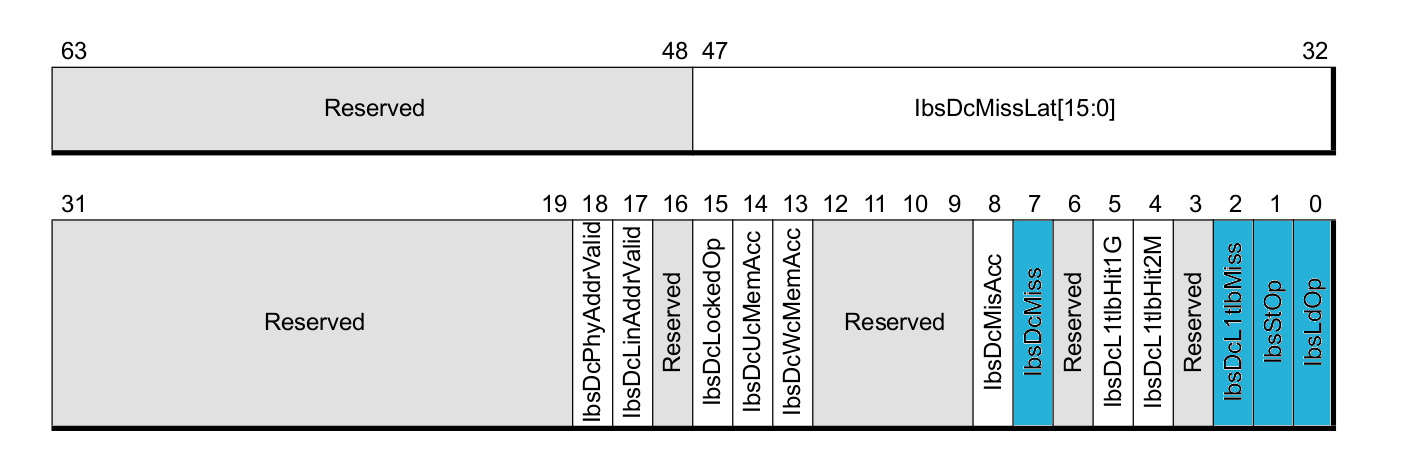
\includegraphics[scale=0.22]{img/data3_color.png}
            \caption{Schéma du registre MSR IbsOpData3}
          \end{figure}
        }
      \end{frame}

    \subsection{Instruction Based Sampling - Défauts}
     \bframe
       \begin{itemize}
         \item overhead: traitement coûteux des mesures
         \item pas de vision d'ensemble
       \end{itemize}
     \end{frame}

    \subsection{Mise en place}
       \begin{frame}{\secname}{\subsecname(1)}        
	\begin{itemize}
 
	  \item les interruptions matérielles - APIC
	  \visible{
            \begin{figure}[h]
              \centering
              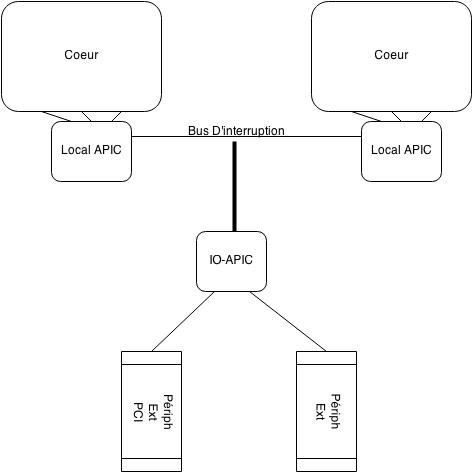
\includegraphics[scale=0.28]{img/apic_diag.jpg}
              \caption{Schéma des composants matériels qui gèrent les interruptions}
            \end{figure}
          }
	  \item<2-> interruptions IBS sont de type NMI (Non Maskable Interrupt)
	\end{itemize}
       \end{frame}

     \begin{frame}{\secname}{\subsecname (2)}        
	Pour configurer les mesures :
	\begin{itemize}
          \item configuration de l'APIC
          \begin{itemize}
            \item informer l'APIC de la présence d'interruptions IBS
            \item à faire pour chaque coeur
          \end{itemize}
          \item enregistrement d'un handler NMI
          \begin{itemize}
            \item appelé à chaque interruption IBS
            \item récolte les informations dans les registres MSR
          \end{itemize}
        \end{itemize}
	\vspace{0.4cm}
        Lancer les mesures (IbsOpCtl) : 
	\begin{itemize}
	  \item configurer le taux d'échantillonnage
	  \item bit IbsOpEn = 1
	  \item à faire sur le coeur du thread concerné
	\end{itemize}
      \end{frame}

    \section{Mesures sur le noyau Linux}
    \subsection{Chaleur d'un thread}
      \bframe
        \begin{itemize}
          \item un compteur représente l'activité d'un thread
          \item différents critères d'activité:
            \begin{itemize}
              \item état: (in)actif
              \item taux d'utilisation mémoire
              \item nombre d'entrées/sorties
              \item commnunications entre threads
              \item \ldots
            \end{itemize}
        \end{itemize}
      \end{frame}

    \subsection{Méthodes de tri envisagées}
      \bframe
        \begin{itemize}
          \item nécessité d'une structure dédiée
          \item utilisation d'un tableau ou d'une liste chainée
          \begin{itemize}
            \item insertion de nouveaux threads
            \item difficulté à trouver les threads morts
            \item tri peu performant
          \end{itemize}
        \end{itemize}
        \visible<2-> {
          \begin{alertblock}{Conclusion}
            Solution abandonnée
          \end{alertblock}
        }
      \end{frame}

      \bframe
          Utilisation d'un tableau de chaleur
          \myfig{0.25}{img/screen1.png}
      \end{frame}
      \bframe
          Utilisation d'un tableau de chaleur
          \myfig{0.25}{img/screen2.png}
      \end{frame}
      \bframe
          Utilisation d'un tableau de chaleur
          \myfig{0.25}{img/screen3.png}
      \end{frame}
      \bframe
          Utilisation d'un tableau de chaleur
          \myfig{0.25}{img/screen4.png}
      \end{frame}

    \subsection{Solution retenue}
      \bframe
        \begin{itemize}
          \item ajout du compteur dans la task\_struct
          \item on conserve le tableau de chaleur précédent
          \item structure Gestion pour les listes
        \end{itemize}
        \myfig{0.3}{img/screen5.png}
      \end{frame}

      \bframe
        \myfig{0.33}{img/screen6.png}
      \end{frame}

    \subsection{Réalisation}

      \bframe
        Algorithme:
        \begin{itemize}
          \item[1] parcourir la task\_struct
          \begin{itemize}
            \item[a] si RUNNING $\rightarrow$ incrémentation du compteur de chaleur
            \item[b] sinon décrémentation
          \item[2] stopper IBS
          \item[3] vider le tableau de chaleurs
          \end{itemize}
          \item[4] générer le tableau de chaleurs
          \item[5] lancer les mesures sur les threads chauds
        \end{itemize}
      \end{frame}

      \bframe
        \begin{block}{Optimisation}
          \begin{itemize}
            \item Utilisation d'un facteur d'incrémentation et de décrémentation
              dynamique
          \end{itemize}
        \end{block}
        \visible<2-> {
          \begin{alertblock}{Problèmes}
            \begin{itemize}
            \item pas d'IBS avec qemu $\rightarrow$ merge impossible sur Magny Cour
            \end{itemize}
          \end{alertblock}
        }
      \end{frame}

  \section{Conclusion}
    \subsection{}
      \bframe
        \begin{block}{Apports personnels}
          \begin{itemize}
            \item beaucoup de connaissances acquises
            \item utile pour l'année prochaine
            \item découverte d'une nouvelle architecture prometteuse
          \end{itemize}
        \end{block}
        \begin{block}{Ce qu'il reste à faire}<2>
          \begin{itemize}
            \item merger les deux parties du projet sur Magny Cour
            \item mettre en place un traitement des données
            \item améliorer l'algorithme de tri d'activités
          \end{itemize}
        \end{block}
      \end{frame}

      %% \bframe
      %%   20/20 ou chinois tuer et manger ta famille !
      %%   \begin{figure}[h]
      %%     \centering
      %%     
\includegraphics[scale=0.4]{img/jackiechan.jpg}\newline
      %%     \textit{``Tu veux un bol de riz ?''}
      %%   \end{figure}
      %% \end{frame}





\end{document}
